\documentclass{article}
\usepackage{amsmath}
\usepackage{pgfplots}
\usepackage{enumitem}
\author{Tianyu Du}
\date{Sep. 2017}
\title{ECO 101 Notes}
\begin{document}
	\maketitle
	\tableofcontents
	\section{Basis: Sep.10 2017}
	\paragraph{Grades}\quad
	\begin{itemize}
	\item Overall: 60\% Term + 40\% Final.
	\item Term Grade:
	\begin{itemize}
		\item Oct(T1) = 23\%
		\item Nov(T2) = 36\%
		\item Warm-up = 1\%
	\end{itemize}
	\end{itemize}
	\paragraph{Topics}\quad
	\begin{itemize}
		\item Basic concepts.
		\item Supply, demand, elasticity. 
		\item Theory of household behaviour. 
		\item Theory of the firm. 
		\item Perfect competition.
		\item Monopoly.
		\item Other Market structures. 
		\item Issues/Role of government.
	\end{itemize}
	\section{Lecture Assessment \#1: First Principles.}
	\paragraph{Sep.10 2017}
	\paragraph{Topics}
	\begin{itemize}
		\item Choices. 
		\item Scarcity. 
		\item Resources. 
			\begin{itemize}
				\item Natural. Land.
				\item Human. Labour.
				\item Capital. Capital.
			\end{itemize}
		\item Outputs. 
		\item entrepreneurship.
	\end{itemize}
	\paragraph{Areas}
	\begin{itemize}
		\item Micro: Individual decision making.
			\begin{itemize}
				\item Households / Consumers.
				\item Firms / Producers.
			\end{itemize}
		\item Macro: Economy as the aggregate.
	\end{itemize}
	\paragraph{Major questions}
	\begin{itemize}
		\item What.
		\item How.
		\item For whom.
	\end{itemize}
	\section{Production possibility curve(PPC)}
	\paragraph{Assumptions}
	\begin{enumerate}
		\item 2 goods.
			\begin{itemize}
				\item Civilian.
				\item Military.
			\end{itemize}
		\item Limited resources.
		\item Technology given.
	\end{enumerate}
	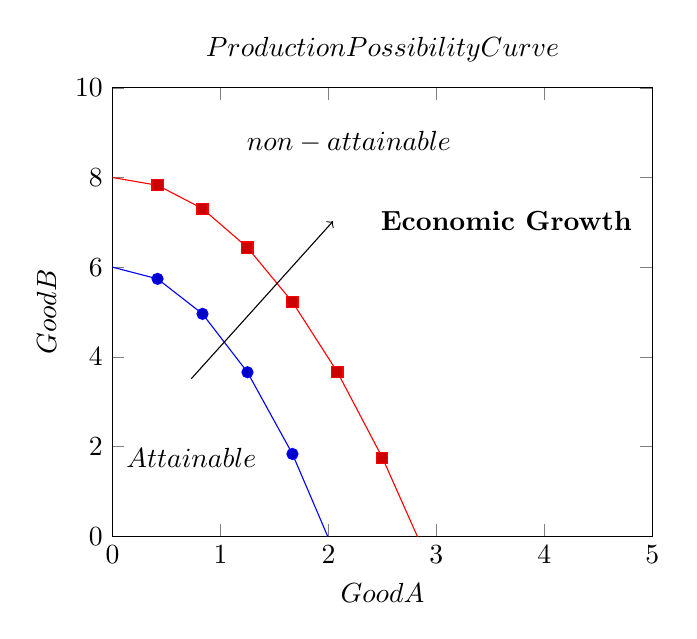
\begin{tikzpicture}
	\begin{axis}[xlabel=$Good A$,ylabel=$Good B$,title=$Production Possibility Curve$,
	xmin = 0,
	xmax = 5,
	ymin = 0,
	ymax = 10,
	]
	\addplot(x,6 + -1.5 * x ^ 2);
	\addplot(x,8 + -1 * x ^ 2);
	\end{axis}
	\node at (3,5) {$non-attainable$};
	\node at (1,1) {$Attainable$};
	\draw[->] (1,2) -- (2.8,4);
	\node at (5,4) {\textbf{Economic Growth}};
	\end{tikzpicture}
	\section{Gains from Trade}
	\paragraph{Assumptions}
	\begin{itemize}
		\item 2 Goods.
		\item 2 Countries.
	\end{itemize}
	\paragraph{Models}
	\begin{itemize}
		\item Absolute advantages.
		\item Comparative advantages.
	\end{itemize}
	\paragraph{Productions and Opportunity costs}
	\begin{center}
		\begin{tabular}{|c|c|c|}
			\hline
			Capacity(O.C.) & Wheat & Vodka \\ \hline
			Canada & 30(1/6 V) & 5(6 W) \\ \hline
			Russia & 10(2 V) & 20(1/2 W) \\
			\hline
		\end{tabular}
	\end{center}
	\paragraph{Example 2}
	\quad \newline Canada got absolute advantages in \emph{both} production.
	\newline Canada got comparative advantage in wheat, and Russia got comparative advantage in Vodka.
	\begin{center}
		\begin{tabular}{|c|c|c|}
		\hline
			Capacity(O.C.)& Wheat & Vodka \\ \hline
			Canada & 30(2/3 V) & 20(3/2 W) \\ \hline
			Russia & 10(1 V) & 10(1 W) \\ \hline
		\end{tabular}

	\end{center}
\end{document}















